\originalchapter{研究生作业三：界面与波包}
题面据8.311作业3全部5题, 解答为AI独立推导并与官方解答对照. 本章静态介质为线性、均匀、各向同性, 无自由界面荷流时才使用所列折线规律.
\originalsection{介质边界与场线折向}
\begin{exercise}
原题1. (a) 从Maxwell方程导出界面条件; (b) 静电介质交界无自由面荷时求电场线法线夹角关系; (c) 无自由面流时求静磁场线关系.
\end{exercise}
\begin{solution}
跨界薄柱给$\nn\cdot(\vct D_2-\vct D_1)=\sigma_f$、$\nn\cdot(\bb_2-\bb_1)=0$; 缩小矩形环给$\nn\times(\ee_2-\ee_1)=0$、$\nn\times(\vct H_2-\vct H_1)=\vct K_f$. 若$\sigma_f=0$, 则$\varepsilon_1E_{1n}=\varepsilon_2E_{2n}$、$E_{1t}=E_{2t}$, 所以$\tan\theta_2=(\varepsilon_2/\varepsilon_1)\tan\theta_1$. 若$\vct K_f=0$, 同理$H_{1t}=H_{2t}$、$\mu_1H_{1n}=\mu_2H_{2n}$, 得$\tan\theta_2=(\mu_2/\mu_1)\tan\theta_1$. 后者亦为$B$方向的角关系. 法向为零等退化情况直接用分量条件解释.
\end{solution}
\originalsection{平面镜像：电荷、电偶极、磁偶极}
\begin{exercise}
原题2. (a) 点电荷位于真空侧距介质平面$a$, 求势及受力; (b) 任意取向电偶极; (c) 将问题推广为磁偶极与磁性半空间.
\end{exercise}
\begin{solution}
界面$z=0$, 上方真空, 下方介电率$\eps\varepsilon_r$. 把像荷放$z=-a$, 上方$V=q/(4\pi\eps R_+)+q'/(4\pi\eps R_-)$, 下方$V=q''/(4\pi\eps\varepsilon_r R_+)$. 界面$V$连续及$D_n$连续给$q'=\alpha q$、$q''=2\varepsilon_rq/(1+\varepsilon_r)$, $\alpha=(1-\varepsilon_r)/(1+\varepsilon_r)$. 原荷受力$F_z=\alpha q^2/(16\pi\eps a^2)$, 正$z$远离界面.

(b) 由两相反荷的小距离极限, $\pp'_{\parallel}=\alpha\pp_{\parallel}$, $p'_z=-\alpha p_z$. 在源位置算像场, $\ee_{\rm img}=-\alpha(\pp_\parallel+2p_z\hat{\vct z})/(32\pi\eps a^3)$. 保持偶极矩不随$a$改变, 像响应能是$U=-\pp\cdot\ee_{\rm img}/2=\alpha(p_\parallel^2+2p_z^2)/(64\pi\eps a^3)$, 所以$F_z=3\alpha(p_\parallel^2+2p_z^2)/(64\pi\eps a^4)$. 二分之一来自逐渐建立诱导源, 不能把随$a$移动的像偶极当外部固定偶极来算能量.

(c) 磁标势同样匹配$H_t,B_n$, 令$\alpha_m=(1-\mu_r)/(1+\mu_r)$及$\pp\to\mm$, 得$m'_\parallel=\alpha_m m_\parallel$, $m'_z=-\alpha_m m_z$及$F_z=3\mu_0\alpha_m(m_\parallel^2+2m_z^2)/(64\pi a^4)$. 磁矩源区之外才能采用无旋$H$势.
\end{solution}
\originalsection{一维波动方程及边界反射}
\begin{exercise}
原题3. 波速$v>0$. (a) 证明$f=f_R(x-vt)+f_L(x+vt)$; (b) 从$f(x,0)=F_1(x)$、$\partial_tf(x,0)=F_2(x)$求解; (c) 半轴$x>0$端点$f(0,t)=0$, 高斯包入射并反射, 绘$t<0,0,>0$形状; (d) 改边界为$\partial_tf(0,t)=u\partial_xf(0,t)$, 求反射并讨论$u$大小.
\end{exercise}
\begin{solution}
(a) 令$\xi=x-vt,\eta=x+vt$, 方程变为$\partial_\xi\partial_\eta f=0$, 两次积分得左右行波. (b) 初值分别给$f_R+f_L=F_1$、$v(f'_L-f'_R)=F_2$, 积分后
$ f(x,t)=[F_1(x-vt)+F_1(x+vt)]/2+(2v)^{-1}\int_{x-vt}^{x+vt}F_2(s)\dd s$.

(c) 取入射$f_L(\eta)=e^{-\eta^2}$（长度已归一）, 则$f_R(\xi)=-e^{-\xi^2}$, 总场$f=e^{-(x+vt)^2}-e^{-(x-vt)^2}$在端点恒零. 图画$v|t|=2$、$t=0$及反射后, 整包反号而非能量消失.
\begin{center}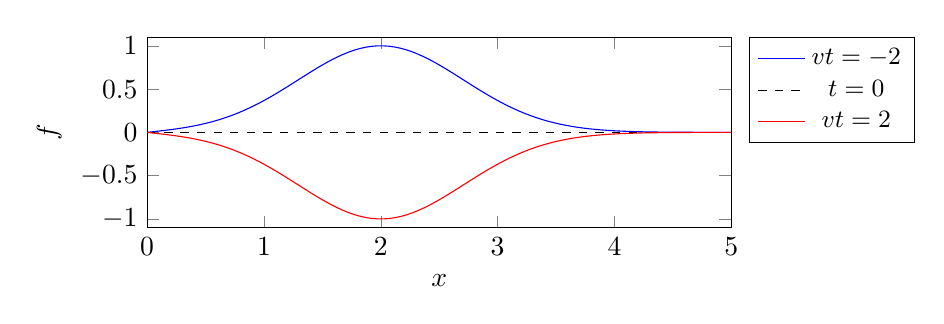
\begin{tikzpicture}\begin{axis}[width=9cm,height=4cm,xmin=0,xmax=5,ymin=-1.1,ymax=1.1,xlabel={$x$},ylabel={$f$},legend style={font=\small,at={(1.03,1)},anchor=north west}]
\addplot[blue,domain=0:5,samples=100]{exp(-(x-2)^2)-exp(-(x+2)^2)};\addlegendentry{$vt=-2$}
\addplot[dashed,black,domain=0:5]{0};\addlegendentry{$t=0$}
\addplot[red,domain=0:5,samples=100]{exp(-(x+2)^2)-exp(-(x-2)^2)};\addlegendentry{$vt=2$}
\end{axis}\end{tikzpicture}\end{center}
(d) 在端点代入导数给$(v+u)f'_R(-vt)=(v-u)f'_L(vt)$; 对自变量积分并令无独立常背景, 得$f_R(\xi)=\eta f_L(-\xi)$、$\eta=(u-v)/(u+v)$. 被动边界$u\ge0$时$u<v$反号、$u>v$同号、$u=v$无反射, $u=0$回到端点固定情形. $u=-v$是奇异边界, 不能用此公式; $u<0$可能引入主动能量输入.
\end{solution}
\originalsection{任意初始电磁包的左右分解}
\begin{exercise}
原题4. 真空$t=0$时$\ee=E_0f(z)\hat{\vct x}$、$\bb=B_0f(z)\hat{\vct y}$. 其中$f(z)=e^{-az^2}$、$a>0$. 求能量、动量密度及其比、随后传播, 各方向能量占多少? 哪种初值仅单向传播?
\end{exercise}
\begin{solution}
$u=\eps(E_0^2+c^2B_0^2)f^2/2$, $g_z=\eps E_0B_0f^2$. 一般$g_z/u=2E_0B_0/(E_0^2+c^2B_0^2)$. 单位截面总能及总动量分别乘$\int e^{-2az^2}\dd z=\sqrt{\pi/(2a)}$. 单向波须$E_0=\pm cB_0$, 此时$g_z/u=\pm1/c$. 一般令$A_\pm=(E_0\pm cB_0)/2$, 则$E_x=A_+f(z-ct)+A_-f(z+ct)$, $B_y=[A_+f(z-ct)-A_-f(z+ct)]/c$. 相加还原初值, 每项满足Maxwell. 正、负行波能量$U_\pm=\eps A_\pm^2\int f^2\dd z$, 比例$(E_0\pm cB_0)^2/[2(E_0^2+c^2B_0^2)]$. 即使两包重叠, 总能中的交叉项也因电磁项符号相反而消去.
\end{solution}
\originalsection{正入射介质与反向入射}
\begin{exercise}
原题5. 真空$x>0$与无损非磁介质$x<0$平面交界. (a) 写两侧一维波方程及界面条件; (b) 消去介质形成真空侧Robin边界, 构造反射/透射包; (c) 求从介质反向入射的场幅、传播速度与功率系数. 原卷的$90^\circ$是相对界面而非相对法线.
\end{exercise}
\begin{solution}
(a) 取$E_y,B_z$, 真空$E_{xx}-E_{tt}/c^2=0$, 介质$E_{xx}-n^2E_{tt}/c^2=0$, $n=\sqrt{\varepsilon_r}>0$. 界面$E_y,B_z$连续. (b) 下方只有向负$x$透射波, $B_z=-nE_y/c$; 由Faraday $\partial_tB_z=-\partial_xE_y$, 在界面真空侧亦有$\partial_tE_y=(c/n)\partial_xE_y$. 这正是题3的$u=c/n$边界, 取$v=c$给反射系数$(1-n)/(1+n)$. 设输入时间包$F$, 则真空$E_y=F(t+x/c)+rF(t-x/c)$, 介质$E_y=t_0F(t+nx/c)$, $t_0=1+r$. 同时$B_z$分别为$[-F(t+x/c)+rF(t-x/c)]/c$及$-nt_0F(t+nx/c)/c$. 因而两场界面条件均已逐点实现.\par
(c) 波阻抗$Z_2=Z_0/n$. 法场切向连续给$1+r=t$、$(1-r)/Z_1=t/Z_2$, 所以从真空入射$r=(1-n)/(1+n)$、$t=2/(1+n)$; 反向$r=(n-1)/(n+1)$、$t=2n/(n+1)$. 反向介质包为$F(t-nx/c)+rF(t+nx/c)$, 真空透射为$t_0F(t-x/c)$, 对应界面切向电场匹配. 两方向的功率反射均$R=(n-1)^2/(n+1)^2$, 透射均$T=4n/(n+1)^2$, $R+T=1$. 介质速$c/n$, 真空$c$; 频率连续而空间波长改变. 对窄包无色散时以同一时间函数$f(t-z/v)$匹配, 则振幅按$r,t$改变、持续时间不变、空间长度随$v$改变.
\end{solution}
